\chapter{Approach}

\section{Implementation Overview}

\begin{figure}[ht]
\caption{Implementation overview}
\label{fig:implementation-overview}
\centering
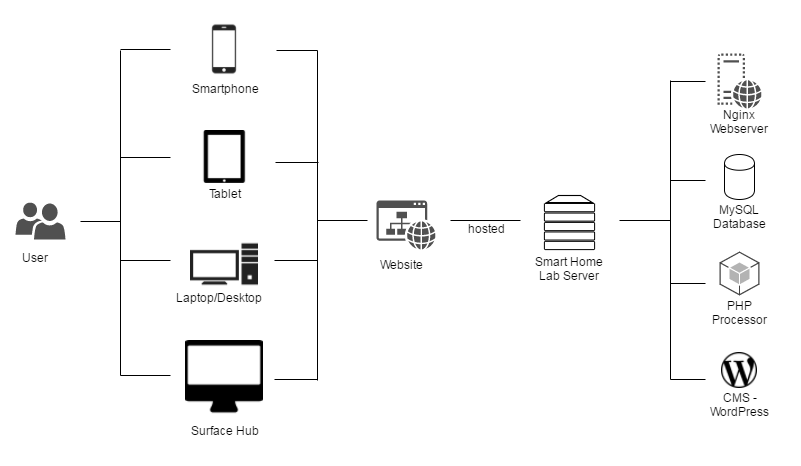
\includegraphics[width=\linewidth,keepaspectratio]{approach/process-diagram.png}
\end{figure}

Figure~\ref{fig:implementation-overview} shows the general implementation of the website for the smart home laboratory. The website is hosted in a physical server, which is located inside the smart home laboratory. This physical server is running the operating system, Ubuntu Server 16.04.2 LTS. In this server, the following software have been installed. They are Nginx HTTP or web server, MySQL database server, PHP application server and WordPress. The website is accessible by various devices by users.

\begin{figure}
\caption{The main components of the website}
\label{fig:use-cases-diagram}
\centering
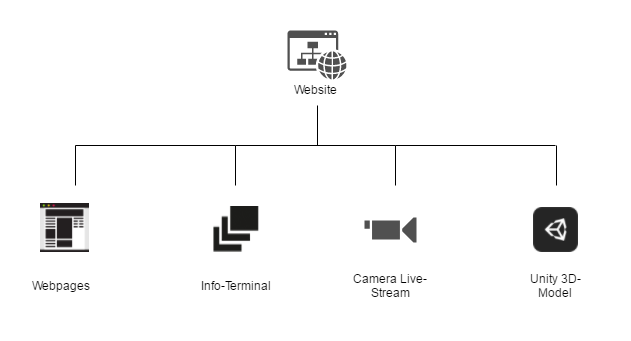
\includegraphics[width=.85\linewidth,keepaspectratio]{approach/use-cases-diagram.png}
\end{figure}

The website in general consists of four parts as shown in Figure~\ref{fig:use-cases-diagram}. They are:
\begin{description*}
\item[Web pages] represent normal web pages such as Home, About, Components, Panels etc.
\item[Info-Terminal] a full screen web page with slider that displays an automated tour
\item[Live Stream] a web page that has been embedded with live video stream and controllers of an IP Camera
\item[3D-Model] a web page that has been integrated with Unity 3D-Model
\end{description*}

\section{Web Pages}
\subsection*{Header}
The web pages are designed with the header consisting of main navigation menu. To the left of main navigation menu, the logo of the institution can be found. To the right of the main navigation menu, a downward arrow can be found. The logo will take user the home page, where else the downward arrow will slide the web page to content part.

\subsection*{Single Column View}
The main body part is programmed to be single column view. The reason is to minimize clutters and distractions through widgets or banners, and at the same time to give extra focus and emphasize on the main contents.

\subsection*{Sectioning}
The web pages has been separated by sectioning. Each section has been equipped with two arrows -- downward and upward. The idea here is  to display a similar group of information in one section. Each section are sized to fit the screen size of HD and FHD screens.

\subsection*{Navigation Arrows}
As mentioned before, each section has two arrows to assist the user to navigate from one section to another. By clicking the upward button will scroll the page automatically to previous section, and clicking the downward button will scroll the web page to next section automatically.

\subsection*{Footer}
Another aspect of the web pages is the footer. The footer as the name itself suggest is to be found at the end of every web page. The footer is divided into two sections. The left section of the footer consists of the copyright statement. The right section of the footer contains a link to \emph{Impressum} page.

\section{Info-Terminal}
\subsection*{Full-Screen Mode}
The info-terminal is programmed to work optimally in full screen mode. It is the only web page, where the header and footer have been removed. The info-terminal consists of only the body part filling the whole screen from left to right and top to bottom.

\subsection*{Screen Ratio}
The info-terminal has been sized to the ratio of 16:9. The reason for choosing the ratio 16:9 is, most of devices' screen are built in this ratio. For example, the Full-HD screen with resolution 1920 x 1080 pixel and HD screen with the resolution 1366 x 768 pixel have this ratio. According to \cite{screen-stat}, this screen ratio counts to more than 50\% of the used devices as of July 2017. It has found to be wiser and reasonable to choose this screen ratio.

\subsection*{Screen Size}
The screen size of info-terminal is designed with a resolution of 1920 x 1080 pixel. The reason behind sizing it at this resolution is the Microsoft Surface Hub has the same resolution. As the info-terminal main designing targeting to be used on the Surface Hub, it has been sized at this resolution. However, it has been programmed to responsive, which allows it to resize itself according to fit screens of other resolutions.

\subsection*{Autoplay}
The info-terminal slider has been equipped with autoplay functionality. The autoplay functionality is turned on by default. It is also possible to switch it off, or on, by using the play button located at the top right of the screen.

\subsection*{Navigating}
The info-terminal can be navigate on its own on autoplay mode. Additionally, users can navigate it manually on their own. Here, they can use the left and right arrows which can be found on the left and right edges respectively. Other than that, the slider can be swiped as well in order to perform the navigation.

\subsection*{Thumbnails}
The thumbnails are one of the feature in the info-terminal. The thumbnails are located at the footer of the slider. Users can see the snipped of the slide on the thumbnails and jump to the slide by clicking it. The thumbnails strip aren't designed with swipe functionality as it conflicts with swipe action on the main slider view.

\subsection*{Home Button}
To the top left of the screen, a home button has been placed. This button will take the user to home page. As the info-terminal doesn't have the header, which contains the main navigation menu, it is essential to provide a button that users back to the home page.

\subsection*{Breadcrumb}
Breadcrumb is the hierarchical navigation link which will be displayed as the user navigate from one level to to another. Breadcrumbs gives user a hint on which level they are right as well as letting them jump to higher level with a single click.

\subsection*{Location Map}
On the bottom left of the info-terminal, a small lab image has been added. This image displays the location where the components that are being displayed on the current slide can be found in the lab.

\section{Live Stream}
\subsection*{Security Login}
In order to view the live stream of the camera, the web page has been programmed to request the users to provide the IP address, username and password at the beginning. This is to ensure the safety and privacy. Hence, a HTML form has been designed with three fields for each information together with a submit button. Upon submission, the provided information will be validated.

\subsection*{Live Footage}
The live footage has been embedded into HTML multimedia tag. It has been programmed to continuously request for the latest footage from the IP Camera and update the screen as soon as the response footage has been received. The communication happens asynchronously in background.

\subsection*{Controllers}
In addition to viewing the live footage, users also can control the IP camera. For this purpose, nine buttons, each containing an arrow to where the camera should move, have been designed and added to the web page. Using this button, users can control the camera in real time. For each of this button, JavaScript and AJAX programming has been added to communicate with the IP camera.


